
\documentclass{article}

\usepackage[left=1.8cm,right=1.8cm, top=2cm, bottom = 2cm]{geometry}
\usepackage{amsfonts}

\usepackage{amsmath}
\usepackage{xcolor}

\usepackage{tikz}
\usepackage{subfigure}

\usepackage{pgfplots}

\pgfplotsset{compat=1.10}
\usepgfplotslibrary{fillbetween}
\usetikzlibrary{patterns}



\pagestyle{empty}

\setlength{\tabcolsep}{15pt}


\newcommand{\deriv}[3][]{\frac{\mathrm{d}^{#1}#2}{\mathrm{d}#3^{#1}}}
\newcommand{\diff}{\;\mathrm{d}}

\newcommand{\norm}[1]{\left|\kern-1pt\left|#1\right|\kern-1pt\right|}
\newcommand{\bra}[1]{\left\langle #1 \,\right|}
\newcommand{\ket}[1]{\left|\, #1\right\rangle}
\newcommand{\braket}[2]{\left\langle #1 \mid #2 \right\rangle}




\begin{document}

\title{Harmonic Motion and Damping}
\date{}

\maketitle
\thispagestyle{empty}

\Large

\vskip -10mm

\textbf{\underline{Objective: To understand the three damping regimes for a}}

\textbf{\underline{harmonic oscillator.}}



\vspace{5mm}



\textbf{Recap: RLC Circuits:}\bigskip


Consider a resistor $R$, inductor $L$, and capacitor $C$ in series, connected to a voltage supply, as shown:

\begin{center}
	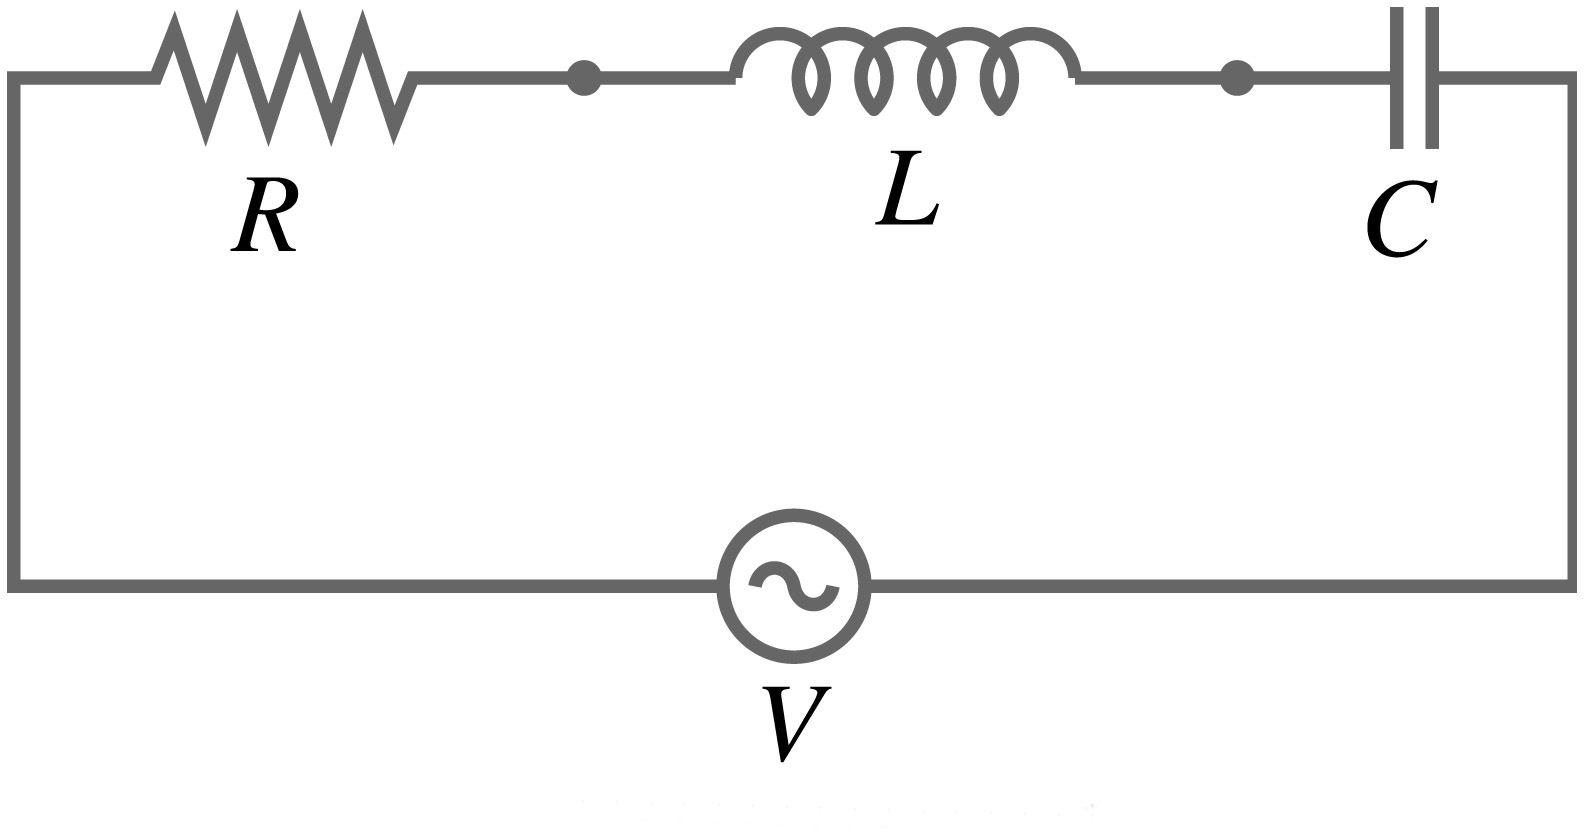
\includegraphics[scale=0.4]{RLC_series_circuit.jpg}
\end{center}

The charge $Q$ on the capacitor is given by $Q=CV_C$, and the rate of change of this charge is the current $I$:
\[I=\deriv{Q}{t}=C\deriv{V_c}{t}.\]
By Ohm's Law,
\[V_r=RI=RC\deriv{V_c}{t},\]
and by Faraday's Law of Induction,
\[V_L=L\deriv{I}{t}=LC\deriv[2]{V_c}{t}.\]
The sum of the three component voltages, $V_C+V_R+V_L$, must be equal to the input voltage $V_\mathrm{in}$, so we have
\begin{align*}
	V_\mathrm{in}&=V_C+RC\deriv{V_C}{t}+LC\deriv[2]{V_c}{t}\\
	\frac{1}{LC}V_\mathrm{in}&=\deriv[2]{V_C}{t} + \frac{R}{L}\deriv{V_C}{t} + \frac{1}{LC}V_C.
\end{align*}

\clearpage


\textbf{Theory: Laplace Analysis of an RLC Circuit:}\bigskip

We have
\[\deriv[2]{V}{t}+\frac{R}{L}\deriv{V}{t}+\frac{1}{LC}V=\frac{1}{LC}f(t),\]
where $f(t)=V){\mathrm{in}}$ and $V=V_C$. To find the transfer function of this, we set $f(t)=\delta(t)$ (for the impulse response) and take the Laplace transform, giving
\[X(s)=\frac{\frac{1}{LC}}{s^2+\frac{R}{L}s+\frac{1}{LC}}.\]

To find poles, we wish to solve
\[s^2+\frac{R}{L}s+\frac{1}{LC}=0.\]
First consider the simpler case when $R=0$, so there is no resistance in the circuit (no damping). Then the denominator is $s^2+\frac{1}{LC}$, which has roots at $\pm\sqrt{\frac{-1}{LC}}$. To simplify this expression, we introduce a new parameter, $\omega_n=\sqrt{\frac{1}{LC}}$, so we can write simply $\pm\omega_nj$ for the poles in the undamped case. This $\omega_n$ is called the \textit{natural frequency} of the system, for reasons which will shortly become apparent.

Now return to the general case, when $R\neq 0$. The roots of the denominator (poles of the transfer function) are found by the quadratic formula/completing the square:
\begin{align*}
	-\frac{R}{L}\pm\frac{1}{2}\sqrt{\frac{R^2}{L^2}-\frac{4}{LC}}&= -\frac{R}{2L}\pm\sqrt{\frac{1}{4}\left( \frac{R^2C}{L^2C}-\frac{4L}{L^2C} \right)}\\
	&=-\frac{R}{2L}\pm\sqrt{ \frac{R^2C-4L}{4L^2C} }\\
	&=-\frac{R\sqrt{C}}{2\sqrt{L}}\sqrt{\frac{1}{LC}}\pm\sqrt{ \frac{1}{LC}\frac{R^2C-4L}{4L} }\\
	&=-\frac{R\sqrt{C}}{2\sqrt{L}}\omega_n \pm \omega_n\sqrt{\left(\frac{R\sqrt{C}}{2\sqrt{L}}\right)^2-1}\\
	&= -\zeta\omega_n \pm \omega_n\sqrt{\zeta^2-1},
\end{align*}
 where we have introduced $\zeta=\frac{R\sqrt{C}}{2\sqrt{L}}$, the \textit{damping ratio}. Going backwards, we see that $\frac{1}{LC}=\omega_n^2$, and $\frac{R}{L}=2\zeta\omega_n$, so the transfer function can be written as
 \[X(s)=\frac{\omega_n^2}{s^2+2\zeta\omega_ns+\omega_n^2}.\]

\clearpage



\textbf{The Undamped Case:}\bigskip

Consider an LC circuit (so $R=0$, we have no damping). Then the differential equation is
\[\deriv[2]{V}{t}+\frac{1}{LC}V=\frac{1}{LC}f(t),\]
and the transfer function is
\[\frac{\frac{1}{LC}}{s^2+\frac{1}{LC}}=\frac{\omega_n^2}{s^2+\omega_n^2}.\]


\begin{enumerate}
	\item Show that $s^2+\omega_n^2=(s+j\omega_n)(s-j\omega_n)$. Note: this can be done either by directly multiplying the given expression out, or by finding the roots of the left-hand side and using the Polynomial Factor Theorem; the first method is quicker, but relies on being given the factorisation to check, whereas the second method lets you find the factorisation for yourself.
	\item Show that the transfer function has partial fractions decomposition
		\[\frac{\omega_n^2}{s^2+\omega_n^2}=\frac{\frac{j\omega_n}{2}}{s+j\omega_n}-\frac{\frac{j\omega_n}{2}}{s-j\omega_n}.\]
	\item Hence show that the impulse response is
		\[H(t)\left(\frac{j\omega_n}{2}e^{-j\omega_n t} - \frac{j\omega_n}{2}e^{j\omega_n t}\right).\]
	\item Hence show that the impulse response is
		\[H(t)\omega_n\sin(\omega_n t).\]
		Hint: $-j=\frac{1}{j}$, and Euler's equation let's you express the sine function in terms of exponentials.
	\item By differentiating $\omega_n\sin(\omega_nt)$, show that for $t>0$ the impulse response satisfies
		\[\deriv[2]{V}{t}+\omega_n^2V = 0.\]
	\item Suppose the inductance is $20\mu\mathrm{H}$ and the capacitance is $50\mu\mathrm{F}$. At what frequency will the LC circuit oscillate when given a unit impulse? What will be the amplitude of the oscillation?
	\item Find the step response of an LC circuit (\textit{i.e.}, the response when $f(t)=H(t)$), both in general and for the specific $L$ and $C$ values in the last question.
\end{enumerate}


\clearpage



\textbf{Theory: Damping:}\bigskip


Consider the general form of the transfer function (in terms of damping ratio and natural frequency),
\[\frac{\omega_n^2}{s^2+2\zeta\omega_ns+\omega_n^2},\]
and its poles, $-\zeta\omega_n\pm\omega_n\sqrt{\zeta^2-1}$, where $\omega_n=\frac{1}{\sqrt{LC}}$ and $\zeta=\frac{R}{2}\sqrt{\frac{C}{L}}=\frac{R}{2L\omega_n}$. We see that $\omega_n$ is a positive real constant, and so is $\zeta$ as long as $R\neq 0$. Therefore the poles of the transfer function consist of a negative real number, $-\zeta\omega_n$, plus or minus a number whichmay be real, zero, or imaginary. So we split into three cases.\bigskip

\textbf{Real, Non-Zero Case:}\smallskip

If $\zeta>1$, then $\zeta^2-1$ is positive, so its square root is real. In this case the two poles of the transfer function are distinct real numbers, say $\alpha$ and $\beta$. Then the denominator factorises as $(s-\alpha)(s-\beta)$, so the partial fractions decomposition will have terms $\frac{A}{s-\alpha}$ and $\frac{B}{s-\beta}$; taking the inverse transform will give us two exponentials, with growth/decay rates $\alpha$ and $\beta$. In fact, they will both be exponential decay terms, because the real poles are both negative.

So if $\zeta>1$, the impulse response is a sum of two exponential decay terms. We call this the \textbf{overdamped} case. Note that it comes about from high values of $R$ and $C$ relative to $L$.\bigskip


\textbf{Zero Case:}\smallskip

If $\zeta=1$, then $\zeta^2-1=0$, so we get two equal poles of the transfer function (\textit{i.e.}, a pole of order 2) at $-\zeta\omega_n=-\omega_n$. Indeed, substituting $\zeta=1$ into the original transfer function, we see it becomes
\[\frac{\omega_n^2}{s^2+2\omega_ns+\omega_n^2}=\frac{\omega_n^2}{(s+\omega_n)^2},\]
so we have a pole of order 2 at $-\omega_n$. We will study this case more on the next page. It is the case of \textbf{critical damping}.\bigskip


\textbf{Imaginary Case:}\smallskip

If $\zeta<1$, then $\zeta^2-1$ is negative, so its square root is imaginary. Then the poles of the transfer function occur at two complex points, with real parts $-\zeta\omega_n$ and imaginary parts $\pm\omega_n\sqrt{1-\zeta^2}$. Note here that $\sqrt{\zeta^2-1}=\sqrt{-(1-\zeta^2)}=j\sqrt{1-\zeta^2}$. We will study this case more shortly, and see that we get two exponentially decaying sinusoids. This is the \textbf{underdamped} case.


\clearpage


\textbf{Critical Damping:}\bigskip

Suppose that $\zeta=1$, so we have critical damping. By the definition of $\zeta$, this means $R=2L\omega_n$, or equivalently $R^2C=4L$. The transfer function in this case is
\[\frac{\omega_n^2}{(s+\omega_n)^2},\]
which is already in partial fractions. From a table of Laplace transforms, the inverse transform of this (hence the impulse response) is
\[H(t)te^{-\omega_n t}.\]

\begin{enumerate}
	\item By differentiating, show that for $t>0$ the impulse response satisfies
		\[\deriv[2]{V}{t}+2\omega_n\deriv{V}{t}+\omega_n^2=0.\]
	\item Suppose the inductance is $2\mathrm{mH}$ and the capacitance is $4\mu\mathrm{F}$. What value resistor is needed to acheive critical damping? What is the natural frequency in this case?
	\item Find the step response of a critically damped system, both in general and for the specific component values in the last question.
\end{enumerate}


\clearpage



\textbf{Underdamped Systems:}\bigskip

Suppose that $\zeta<1$, so we have underdamping. This occurs when $R$ and $C$ are small relative to $L$; more specifically, when $R^2C<4L$, by the definition of $\zeta$. The poles of the transfer function occur at
\[-\zeta\omega_n\pm\omega_n\sqrt{\zeta^2-1}=-\zeta\omega_n\pm j\omega_n\sqrt{1-\zeta^2}.\]

The transfer function itself is
\[\frac{\omega_n^2}{s^2+2\zeta\omega_ns+\omega_n^2}.\]


\begin{enumerate}
	\item Introduce a change-of-variable $r=s+\zeta\omega_n$. Show that, in terms of $r$, the transfer function can be written as
		\[\frac{\omega_n^2}{\left(r-j\omega_n\sqrt{1-\zeta^2}\right)\left(r+j\omega_n\sqrt{1-\zeta^2}\right).}\]
	\item Show that this has partial fraction decomposition
		\[\frac{\frac{j\omega_n}{2\sqrt{1-\zeta^2}}}{\left(r+j\omega_n\sqrt{1-\zeta^2}\right)} - \frac{\frac{j\omega_n}{2\sqrt{1-\zeta^2}}}{\left(r-j\omega_n\sqrt{1-\zeta^2}\right)}.\]
	\item Hence show that the transfer function can be expressed in partial fractions as
		\[\frac{\frac{j\omega_n}{2\sqrt{1-\zeta^2}}}{\left(s+\zeta\omega_n+j\omega_n\sqrt{1-\zeta^2}\right)} - \frac{\frac{j\omega_n}{2\sqrt{1-\zeta^2}}}{\left(s+\zeta\omega_n-j\omega_n\sqrt{1-\zeta^2}\right)}.\]
	\item Hence show that the inverse Laplace transform (the impulse response) is
		\[H(t)\frac{\omega_n}{\sqrt{1-\zeta^2}}e^{-\zeta\omega_n t}\left(\frac{j}{2}e^{-j\omega_n\sqrt{1-\zeta^2}t} - \frac{j}{2}e^{-j\omega_n\sqrt{1-\zeta^2}t} \right).\]
	\item Hence show that the impulse response is
		\[H(t)e^{-\zeta\omega_n t}\sin\left(\omega_n\sqrt{1-\zeta^2}t\right).\]
	\item Suppose the inductance is $2\mathrm{mH}$, the capacitance is $4\mu\mathrm{F}$, and the resistance is $500\Omega$. Find the impulse response in this case.
\end{enumerate}






\end{document}